\chapter{Multi-Agent Systems}
One way to sustain the simulation is to create a simulation process that will feature constant communication with a user of the simulation system.
Describing game characters in terms of their beliefs, intentions and desires is a common way for humans to understand the world and, therefore, a comfortable way to recreate it in a computer simulation. Using agent notion it is possible to create a simulation environment, that would be easily understandable by a human being as well as use existing frameworks to reduce the amount of code, required to make an operable framework and create tests. This chapter provides information on how it can be achieved.\par
\section{Agent Notion}

All agent-oriented software is based on the notion of agent defined in \cite{DUMMY:1}. \par
\theoremstyle{definition}
\begin{definition}{Agent}
    -- computer system that is situated in some environment, and that is capable of autonomous action in this environment in order to meet its delegated objectives.
\end{definition}
After disassembling this definition the list of characteristics that are required by each agent can be created. However, most people use the term ``agent'' when talking about the entity with a bit broader list of characteristics, also known as ``intelligent agent'' \cite{DUMMY:6}. Main characteristics of intelligent agent are:
\begin{itemize}
 \item \textbf{Autonomy}, usually perceived as an ability to operate without direct intervention as well as control over the internal state.
 \item \textbf{Social ability} -- an ability to interact with other agents, usually essential to achieve the goal.
 \item \textbf{Reactivity} -- an ability to receive information from their environment and respond to that information.
 \item \textbf{Proactiveness} -- goal-driven behaviour.
\end{itemize}
In \cite{dummy:1} the multi-agent system is defined as the one that consists of agents, but due to questionable restrictions the definition in this book is a bit different.
\begin{definition}{Multi-agent system}
is any system that includes more than one agent.
\end{definition}
Agents are often being disassembled into 3 parts: perception (receiving and preprocessing the input), decision-making and effectors (responsible for influencing the environment). The structure is shown in Figure \ref{GnomeAgent}. Agents constantly receive information from the environment, process it, then use it to choose the information (depicted as "actions" arrow) they are going to send to the environment. Effectors and sensors are used to formalize and restrain the data that can be passed to and from the environment. \par
    \begin{figure}[h!]
     \begin{center}
      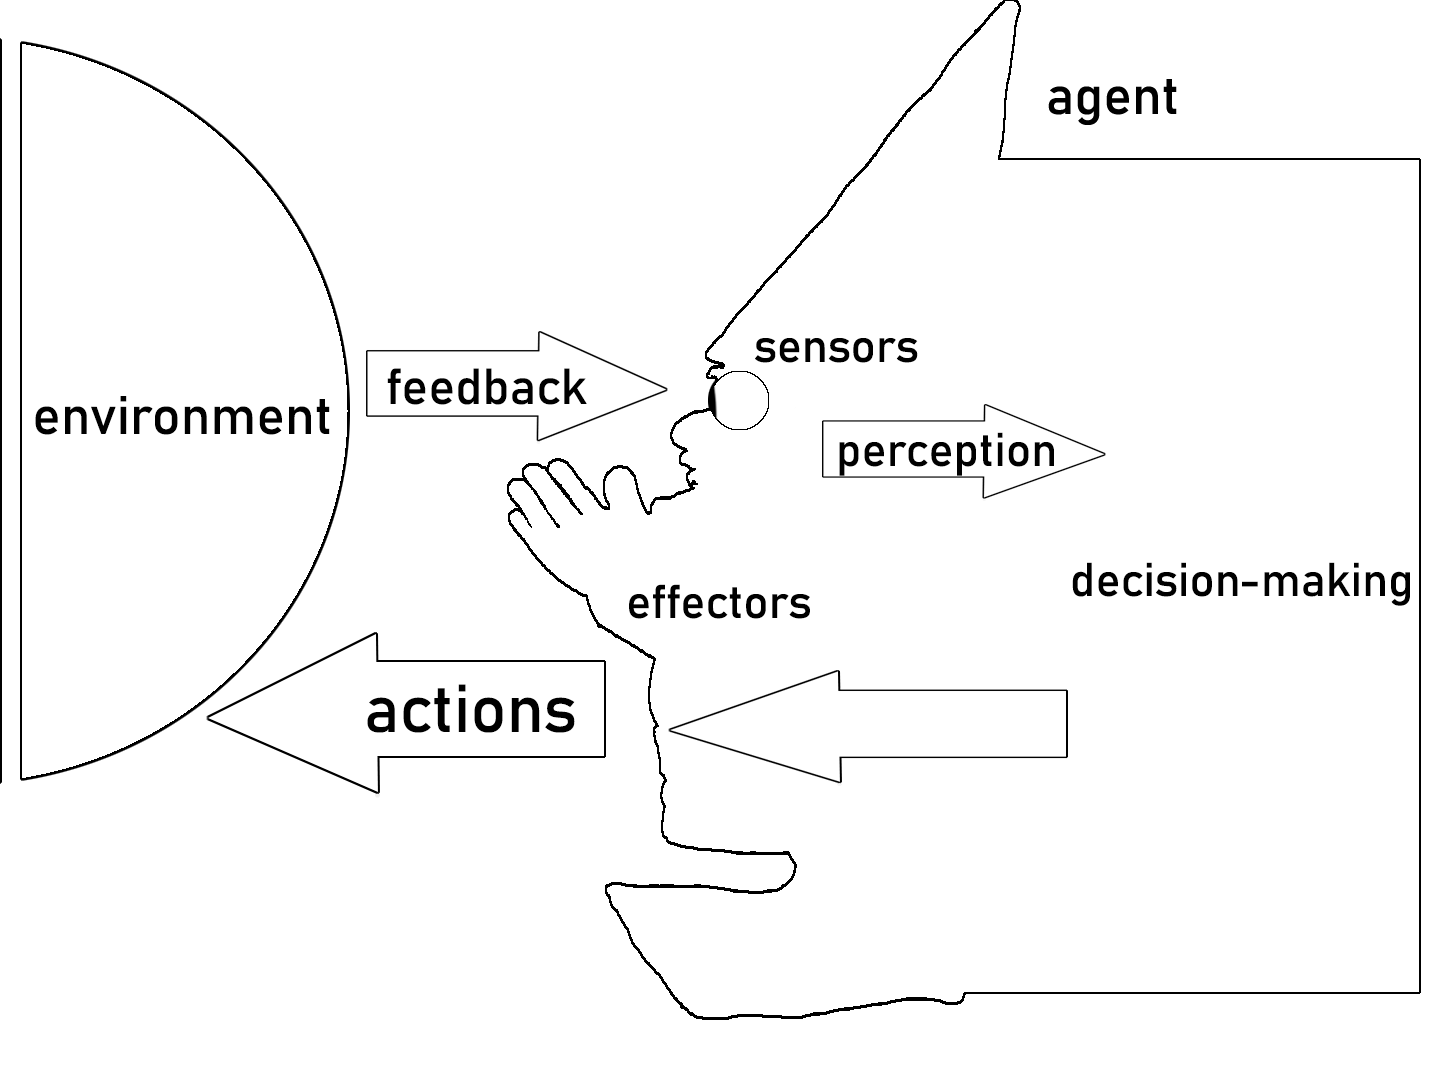
\includegraphics[width=400pt]{gnome_agent}
      \caption{Gnome agent}
      \label{GnomeAgent}
      \end{center}
    \end{figure}
%In classic multi-agent theory agents are being contained by their environment , therefore in any particular moment any agent can interact only with one environment (and, transitively, with other agents in this environment).


\section{Environment}

There is a huge variety in multi-agent systems of functionality that can be provided by the environment. The environment itself can be implemented as one of the agents. On the other hand, it can be used to simplify the structure of all other agents. For example, environment can contain all internal memory of each agent and give their information to them on demand. There are several classifications of environments based on different parameters. Here are some of them according to \cite{DUMMY:1} and \cite{ArtInt}.
\begin{itemize}
\item \textbf{Agent capacity.} Single agent environments are deprived of complexity that is common to multi-agent systems. The main problems that are nonexistent in single agent systems are agent communication and simultaneous access.
\item \textbf{Observability (Accessibility).}  The agent can obtain complete information about the fully observable environment's state in any particular moment. Partially observable environments are a lot more common in the real world. According to \cite{ArtInt} fully observable environment must only provide all the necessary information for the agent to determine the optimal course of actions.
\item \textbf{Determinism.} In deterministic environment the state of the environment is completely determined by the actions of the agent. In any other case it is called stochastic. The only exception given in \cite{ArtInt} is uncertainty that is caused by the actions of other agents.
\item \textbf{Dynamism.} Static environment is guaranteed to preserve its state when no actions are executed by agent. Dynamic environment, on the other hand, usually treats agent's delay of response as idle action. Most multi-agent systems are highly dynamic.
\item \textbf{Discretion.} Discrete environment has finite amount of possible states. Continuous environments usually feature one or more continuous value that rises the number of possible states to infinity. Despite no continuous environments can be created within digital ones, some of the environments.
\item \textbf{Episodicity.} The agent's actions does not affect the observable part of the state in episodic environment. No matter which action is executed by the agent it will not affect any later percepts the agent will be given. The environment that is not episodic is called sequential.
\end{itemize}


\section{Agent Architecture}
Nowadays, there are a lot of agent architectures used in different practical implementations. In this chapter most of the attention is payed to agent's functionality rather than practicality.   That is why this section contains only basic abstract agent architectures. Most of the information in this section was taken from \cite{DUMMY:1}.\par
Consider the environmental instance \(E\), which can be described with finite number of discrete states \(E=\{e,e',...\}\). Now let us assume there is an agent interacting with this environment that can execute one of possible actions  \(Ac = \{\alpha , \alpha' , ... \} \).
A run \(r\) of an agent \(Ag\) in the environment is thus the sequence of interleaved environment states and actions:
\begin{align*}
& r: e_0 \xrightarrow{\text{\(\alpha_0\)}}  e_1 \xrightarrow{\text{\(\alpha_1\)}} e_2 \xrightarrow{\text{\(\alpha_2\)}}... \xrightarrow{\text{\(\alpha_{u-1}\)}} e_u \xrightarrow{\text{\(\alpha_{u}\)}} ... \\
&R\ \text{-- set of possible runs,}\\
&R^{Ac}\ \text{-- subset of}\ R\ \text{with sequences that end with an action,}\\
&R^E\ \text{ -- subset of}\ R\ \text{with sequences, that end with a state,}\\
&\tau\ :\ R^{Ac} \rightarrow 2^E\ \text{-- state transition function,}\\
&Ag\ :\ R^E \rightarrow Ac\ \text{-- generic agent model.}\\
\end{align*}
In this architecture, state transition function maps a run to a set of possible environment states in which the environment might be transferred by the last action from the corresponding run. This formula allows to describe nondeterministic history-dependent environments. The agents, however, must be deterministic.
Here is a simple example.
\begin{example}
 There is a room with a gnome and an apple. The gnome can eat the apple. This environment has 2 states: \(E=\{e,e'\}\), $e$ - apple is in the room, $e'$ - there is no apple in the room.\newline
The only agent in this environment is the gnome. Gnome's actions can be described as
\(Ac = \{\alpha , \alpha'\} \), where
$\alpha$ is to do nothing and
$\alpha'$ is to try to eat the apple. \newline
And the example run would be \(r: e \xrightarrow{\text{\(\alpha\)}}  e \xrightarrow{\text{\(\alpha'\)}} e' \xrightarrow{\text{\(\alpha'\)}} e' \xrightarrow{\text{\(\alpha\)}} e' \).\par
In this run the gnome does nothing during its first turn, then eats the apple, thus changing the environment state. According to the results of this run it might be assumed, that informal specification of agent function would result in eating apple only if the gnome either didn't try to eat or successfully ate the apple on the previous turn.
\end{example}
This architecture is suitable for describing agents with memory thus being able to used for description of any deterministic agent.
The only drawbacks of such approach in designing a real agent are:
\begin{enumerate}
  \item Absence of initial configuration (puts no constraints on the set of describable agents, yet makes overall structure rather complex and sometimes non-intuitive).
  \item Lack of information about the internal structure of an agent.
\end{enumerate}
However, there are subclasses of generic agent that can be described in a simpler / more detailed way \cite{DUMMY:1}.
\begin{itemize}
\item \textbf{Purely reactive agents.} These are basically the agents with no memory. Their decisions to take actions are dependent only on what they've perceived on this turn. They can be described by \(Ag : R\rightarrow Ac\) function and can be easily tested due to being stateless.
\item \textbf{Agents with state.} In this case, we impose restrictions on the internal structure of an agent. Each agent is given a function \(see : E\rightarrow Per\) that determines what part of the environment state the agent can perceive. After information is being perceived, it can influence the internal state $i$ of the agent. This process is described by \(next : I*Per\rightarrow I\). Finally, when the next state is determined, it might trigger one of possible actions \(action: I\rightarrow Ac\). The architecture is depicted in Figure \ref{StateAgent}
    \begin{figure}[h!]
     \begin{center}
      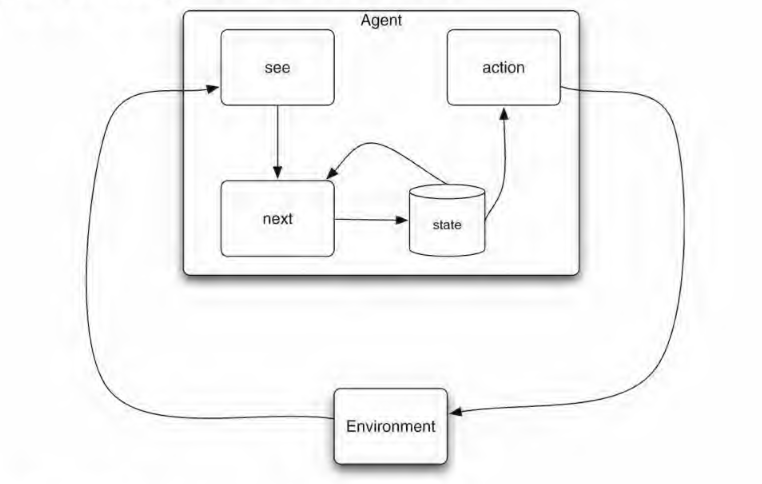
\includegraphics[width=500pt]{agent_with_state}
      \caption{Agent with state.}
      \label{StateAgent}
      \end{center}
    \end{figure}
\end{itemize}
Besides this architectures, there are also less formal and more human-like approaches.
One of them is called BDI (Belief-Desire-Intention) execution model \cite{DUMMY:1}.
BDI architecture uses terms from a folk psychology to describe the agent's behavioral structure. The 4 key concepts of this model are Belief, Desire, Intention and Plan (see Fig.\ref{BDIAgent}). Beliefs represent the agent's internal state. Desires are used by the reasoner (logical part of the agent) to determine the optimal course of actions. Intentions consist of actions that are going to be executed by the agent in order for it to achieve some of its desires. And, finally, plans can be described as long-term composite structures, that encapsulate an enumerated set of actions (intentions), used to simplify the belief system \cite[p.~150]{DUMMY:2}.
    \begin{figure}[h!]
      \begin{center}
      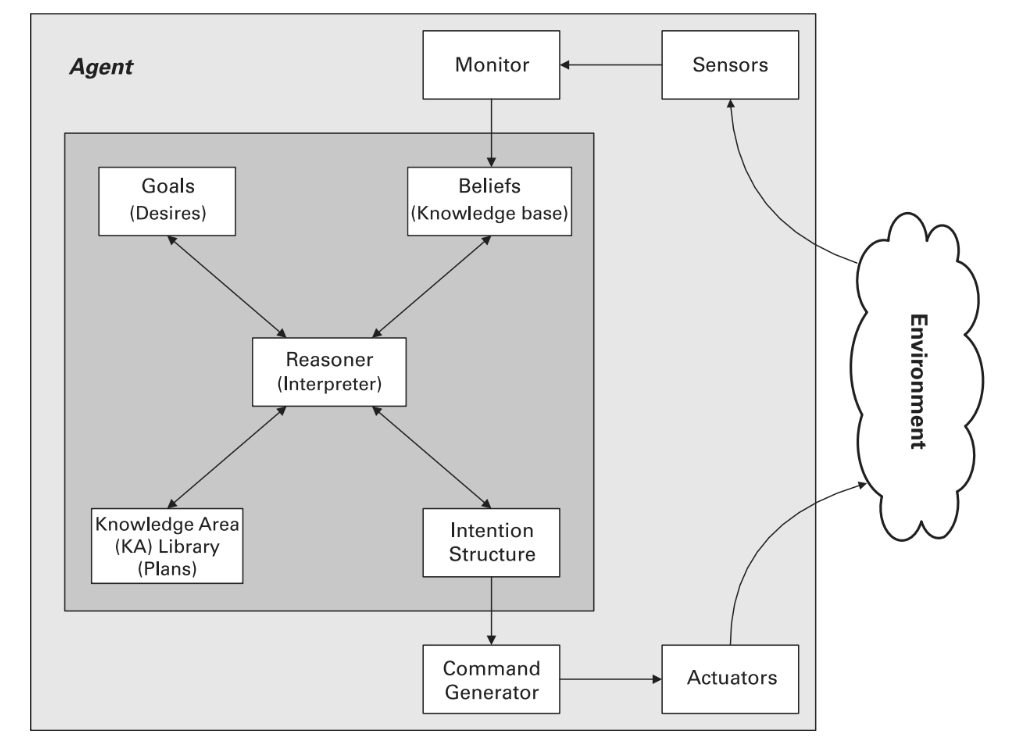
\includegraphics[width=400pt]{BDI}
      \caption{BDI agent architecture.}
      \label{BDIAgent}
      \end{center}
    \end{figure}


\section{Utility Functions}
The essential part of each intelligent agent is goal-driven behaviour.
The most common way to determine the goal of an agent is to specify its utility function \cite{DUMMY:1}.
The perfect utility function result mirrors agent's success of reaching its goals.
The simplest solution is for utility function to evaluate the current state of the environment
(\(u: E\rightarrow \mathbb{R} \)). This kind of utility function proves itself to be inefficient on long-term strategies, but it is still widely used in different fields, such as neural networks. The solution may be for the agent to build a new utility function on top of the given one that will use one's state as an argument. Yet for those who do not want for their agent to feature complex reasoning mechanisms there is a broader class of utility functions which accept the whole run with all the information in it as an argument -- \(u: R\rightarrow \mathbb{R} \).
This is the widest class of utility functions. It features such subclasses as predicates (\(u: R\rightarrow \{0,1\} \)), useful for determining whether the particular goal was achieved.\par
When agent's utility function is constructed, the only thing agent is left to do is to maximize it.
In real environments, which are mostly nondeterministic, highly dynamic and hardly accessible it is possible to operate only with probabilities. For example, sometimes there is no certain answer whether the environment would end up being in a particular state after the agent executes a particular set of actions. Nevertheless, by measuring the probability of this to happen it is still possible to determine the optimal strategy.
Each agent of course might influence the probability of a particular run:
\[\sum_{r \in R(Ag, Env)} P (r| Ag, Env ) = 1,\]
where the \(P (r| Ag, Env )\) is a probability of the run $r$ to happen with agent $Ag$ and the environment $Env$. \(R(Ag, Env)\) is a set of all possible runs of the agent $Ag$ in the environment $Env$.

The concept of  expected utility is described by the next equation:
\[ u_{exp}(Ag,Env)  = \sum_{r \in R(Ag, Env)} u(r) *P (r| Ag, Env ),\]
where $u(r)$ represents the utility value of a particular run.
The optimal agent is considered to be the one that maximizes the expected utility, or
\[ Ag_{opt}(Env)  = \max_{Ag\in AG} u_{exp}(Ag,Env).\]

%\section{Agent types}



\section{Agent Communication}
Agent communication is one of the cornerstones of multi-agent systems. Since each agent is autonomous and features goal-driven behaviour, the overall communication mechanism is much more ``human-like'': instead of executing requests, it becomes more of a deal-making utility-centered conversation. But for that conversation to exist agents at least should understand each other. To make it easier to design the agent communication, different agent communication languages were created. The most popular are FIPA-ACL, KQML and KIF \cite{ap5, DUMMY:1,DUMMY:2,DUMMY:3}.
\subsection{KQML}
KQML stands for Knowledge Query and Manipulation Language.
This language represents a message as an object. Each message has a performative that specifies its type and a list of parameters, which are depicted as ``attribute : value'' pairs.
\begin{center}
\begin{tabular}{|p{1cm} |p{3cm} | p{12cm}|}
\multicolumn{3}{c}{\textbf{Some of KQML attributes}}\\
\hline
\textnumero & \textbf{attribute} & \textbf{meaning} \\
\hline
1&:content    & content of the message \\
\hline
2&:force      & whether the sender of the message will ever deny the content of the message \\
\hline
3&:in-reply   & whether the sender expects a reply, and, if so, an identifier for the reply \\
\hline
4&:reply-with & adding the preferable response specification. \\
\hline
5&:sender     & sender of the message \\
\hline
6&:receiver   & intended recipient of the message\\
\hline
\end{tabular}
\newline
\end{center}
Therefore, a message in KQML may look like this one:
\begin{align*}
(\ & \text{ask-one} \\
  &:content\ (COLOR\ GNOMEHAT\ ?\ color) \\
  &:receiver\ tailor                    \\
  &:language\ LPROLOG                   \\
  &:ontology\ gnome-info\ )             \\
\end{align*}

 ``Ask-one'', in the message above, is a performative. There are around 50 performatives in KQML, each describing the corresponding message type.\par
 The dialogues in KQML can be either synchronous or asynchronous. The types of dialogues are represented on Figure \ref{KQMLDialog}.
    \begin{figure}[h!]
      \begin{center}
     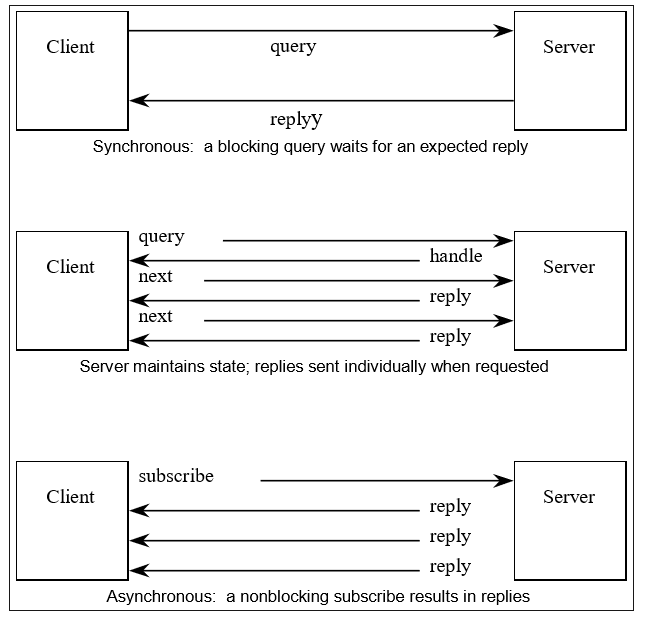
\includegraphics[width=300pt]{kqml}
      \caption{BDI agent architecture.}
      \label{KQMLDialog}
      \end{center}
    \end{figure}

\subsection{FIPA}
Since FIPA ACL was designed for the same purposes as KQML, this two languages have much in common.
The goal behind the creation of the FIPA standard is to utilize it in the development of an agent communication language (FIPA-ACL).  FIPA-ACL is superficially similar to KQML: it defines an ``outer'' language for messages, feature 20 performatives for defining the intended interpretation of messages, and it does not mandate any specific language for message content. In addition, the concrete syntax for FIPA-ACL messages closely resembles that of KQML. For example,the example KQML message from above when encrypted in FIPA-ACL using XML markup language is presented below:
\addtolength{\jot}{-10pt}
\begin{align*}
  &<\text{envelope}> \\
  &\quad <\text{params} index ="1"> \\
  &\quad \quad <\text{to}> \\
  &\quad \quad \quad <\text{agent-identifier}>\\
  &\quad \quad \quad \quad <\text{name}> tailor </\text{name}>\\
  &\quad \quad \quad </\text{agent-identifier}>\\
  &\quad \quad </\text{to}> \\
  &\quad \quad <\text{from}> \\
  &\quad \quad \quad ... \\
  &\quad \quad </\text{from}> \\
  &\quad \quad ...\\
  &\quad </\text{params}>\\
  &</\text{envelope}>\\
  &</\text{message}>\\
  &\quad </\text{performative}>\\
  &\quad \quad ask-one \\
  &\quad </\text{performative}>\\
  &\quad </\text{content}>\\
  &\quad \quad ? \\
  &\quad </\text{content}>\\
  &\quad <\text{ontology}>\\
  &\quad \quad gnome-info \\
  &\quad </\text{ontology}>\\
  &\quad ...\\
  &</\text{message}>\\
\end{align*}

\subsection{KIF}
The knowledge interchange format (KIF) is a simple logic-based language that gained high popularity in  expert systems, databases and intelligent agents. The initial design objective of KIF was to create a ``mediator'' language, useful for translating messages between other languages. The simple example featuring this language is given below.
\begin{center}
\textit{(> (- (length sword) (shaftLength sword)) (- (length knife) (shaftLength knife))) }
\end{center}
This example states that the sword has the longer blade than the knife does.
Despite the existence of this communication protocols there are a lot of cases where it is much more rewarding to create personalized communication protocol for a particular system. However, KQML or FIPA-compliance can make a multi-agent system easily understandable and mergeable with others.

\section{Software Overview}
Since multi-agent systems use to be more complex and are usually less efficient than, for example, systems based only on functional or OOP paradigm, agent oriented programming is not among the popular programming concepts. Nevertheless, due to being used in various scientific researches and AI based systems, agent notion was used in a multiple frameworks and libraries. The comparative table of them can be found in
\textbf{Appendix \ref{appendix:frameworks}}.

The problem with most frameworks is that they were originally designed to fulfill the certain set of tasks: and none of the tasks was similar to the one given in this paper.
Another problem is the commercial license. The most efficient systems have the highest prices. On the other hand there is an ability to completely customize open-source software.

Frameworks that are written to be used with custom or less popular languages are usually the least customizable and are useful only for simulating software, where productivity is of lesser concern than the ability to create the system rapidly.

The leading frameworks (in terms of the quantity of users) are usually implemented for Java or/and C++ programming languages that allows users to customize them in different ways.




